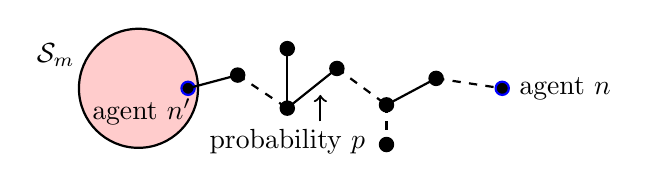
\begin{tikzpicture}[scale=0.42]

    % Main zones
    \filldraw[color=black, fill=red!20, thick] (0,0) circle (1.8cm); % Smaller zone around agent i
    \filldraw[color=blue, fill=black, thick] (1.5,0) circle (0.2); % Agent i
    \filldraw[color=blue, fill=black, thick] (11,0) circle (0.2); % Agent n

    % Intermediate nodes on a zigzag path between i and n
    \filldraw[color=black, fill=black, thick] (3,0.4) circle (0.2);    % Node 1 (slightly above)
    \filldraw[color=black, fill=black, thick] (4.5,-0.6) circle (0.2); % Node 2 (slightly below)
    \filldraw[color=black, fill=black, thick] (6,0.6) circle (0.2);    % Node 3 (slightly above)
    \filldraw[color=black, fill=black, thick] (7.5,-0.5) circle (0.2); % Node 4 (slightly below)
    \filldraw[color=black, fill=black, thick] (9,0.3) circle (0.2);    % Node 5 (slightly above)

    % Dotted line segments connecting nodes from agent i to agent n
    \draw[color=black, thick] (1.5,0) -- (3,0.4);
    \draw[color=black, thick,dashed] (3,0.4) -- (4.5,-0.6);
    \draw[color=black, thick] (4.5,-0.6) -- (6,0.6);
    \draw[color=black, thick, dashed] (6,0.6) -- (7.5,-0.5);
    \draw[color=black, thick] (7.5,-0.5) -- (9,0.3);
    \draw[color=black, thick,dashed] (9,0.3) -- (11,0);

    % Branching nodes
    \filldraw[color=black, fill=black, thick] (4.5,1.2) circle (0.2); % Branch above
    \draw[color=black, thick] (4.5,-0.6) -- (4.5,1.2);

    \filldraw[color=black, fill=black, thick] (7.5,-1.7) circle (0.2); % Branch below
    \draw[color=black, thick, dashed] (7.5,-0.5) -- (7.5,-1.7);

    % Arrow pointing to a dotted line segment with probability label
    \draw[->, thick] (5.5,-1.) -- (5.5,-0.2);
    \draw node at (4.5,-1.6) {probability $p$};

    % Labels
    \draw node at (-2.5,1) {$\mathcal S_m$};
    \draw node at (0.1,-0.7) {agent $n'$};
    \draw node at (12.9,0) {agent $n$};

\end{tikzpicture}